\documentclass[12pt,conference]{IEEEtran}
\IEEEoverridecommandlockouts

% Body font: Cambria 12 pt. Cambria is used where it is installed (XeLaTeX/LuaLaTeX); otherwise Caladea, a free
% font that is metric-compatible with Cambria (same widths and line breaks).
\usepackage{iftex}
\ifPDFTeX
  \usepackage[T1]{fontenc}
  \usepackage{caladea}
\else
  \usepackage{fontspec}
  \IfFontExistsTF{Cambria}{\setmainfont{Cambria}}%
    {\setmainfont{Caladea}[Extension=.ttf, UprightFont=*-Regular, BoldFont=*-Bold, ItalicFont=*-Italic,
                           BoldItalicFont=*-BoldItalic]}
\fi
\usepackage{cite}
\usepackage{amsmath,amssymb}
\usepackage{graphicx}
\usepackage{booktabs}
\usepackage{multirow}
\usepackage{array}
\usepackage{xcolor}
\usepackage{tikz}
\usetikzlibrary{positioning,arrows.meta,fit,backgrounds}
\usepackage[hidelinks]{hyperref}
\usepackage{url}

\newcommand{\pp}{\,pp}
\renewcommand{\arraystretch}{1.08}
\raggedbottom   % no stretched vertical space between paragraphs and headings

\begin{document}

\title{Sentinel-1-Only Land Use and Land Cover Segmentation: Generalisation Limits, Radar-Separable Classes and a
Monthly Change-Monitoring Prototype}

\author{\IEEEauthorblockN{Namrata Bhoyar}
\IEEEauthorblockA{SRH University, Germany}}

\maketitle

\begin{abstract}
Optical satellites cannot observe the ground through clouds, which limits monthly land use and land cover (LULC)
mapping in many regions. This work studies how far synthetic aperture radar alone can replace them. A global dataset
of Sentinel-1 monthly composites with Dynamic World labels was built for 40 study areas on six continents, split by
region and by time (training 2023--24, testing on nine unseen regions in 2025--26). Ten deep-learning models were
trained with an identical protocol: a baseline CNN, a U-Net, DeepLabV3+ with ResNet50, six DeepLabV3+ variants with
deeper or more efficient encoders and an atrous-encoder design, and a multi-temporal DeepLabV3+. Spatial context and
ImageNet pretraining improve the test mIoU from 0.20 to 0.30, but larger encoders and temporal input do not improve it
further, although the same models reach 0.56--0.58 mIoU on the training regions in the test period. The analysis
shows that most errors fall into two class pairs that C-band backscatter cannot separate physically, bare ground versus
snow/ice and cropland versus rangeland. Merging them into a radar-separable six-class scheme raises the overall
accuracy of the same predictions from 0.51 to 0.72. A prototype derives twelve monthly maps, class shares and changes
for any location; a case study of Munich agrees with the independent Esri land-cover map on 87.9\,\% of the pixels and
illustrates how seasonal effects and systematic classification errors affect the calculated change.
\end{abstract}

\begin{IEEEkeywords}
Sentinel-1, synthetic aperture radar, land use and land cover, semantic segmentation, DeepLabV3+, domain
generalisation, change detection, Google Earth Engine
\end{IEEEkeywords}

% =====================================================================================================
\section{Introduction}

Land use and land cover maps are a basic input for monitoring urban growth, deforestation, agriculture and
flooding. Recent global products such as Dynamic World~\cite{brown2022dynamic} and the Esri 10\,m Annual LULC
map~\cite{karra2021global} are derived from Sentinel-2 optical imagery with deep learning. Optical sensors, however, see nothing through clouds or at night, so in the tropics, in monsoon
regions and in northern winters a monthly map often cannot be produced at all. Synthetic aperture radar (SAR) such as
Sentinel-1~\cite{torres2012gmes} transmits its own microwave pulse and observes the surface independently of weather
and illumination. The price is a signal that is harder to interpret: backscatter depends on surface roughness,
geometry and moisture rather than on colour~\cite{ulaby2014microwave}, and it is corrupted by speckle.

This work investigates LULC segmentation that uses Sentinel-1 as its \emph{only} input, and the use of such maps to
quantify monthly change. The study is organised around three questions: (i)~which network design is suitable, (ii)~how
well a model trained on some regions transfers to unseen regions and to a later period, and (iii)~what limits the
accuracy and how reliable the derived change statistics are. The contributions are:
\begin{itemize}
\item a global Sentinel-1/Dynamic World dataset of 40 study areas on six continents with a split by region and by
time, built entirely in Google Earth Engine~\cite{gorelick2017google} and published for reuse;
\item a controlled comparison of ten segmentation models, from a small CNN to DeepLabV3+ variants with up to 75\,M
parameters and a multi-temporal input, all trained with the same protocol and diagnosed for under- and overfitting;
\item evidence that the limiting factors are geographic diversity of the training data and the optical origin of the
class scheme, not network capacity, and a radar-separable six-class evaluation that raises the overall accuracy from
0.51 to 0.72 without retraining;
\item a prototype that maps any location over twelve months, reports class shares and changes in percentage points,
flags unreliable months and compares the result with an independent map, demonstrated in a case study of Munich.
\end{itemize}

% =====================================================================================================
\section{Related Work}

\textit{SAR land-cover mapping.} Multi-temporal Sentinel-1 series are
effective for crop-type mapping because the phenological cycle changes backscatter over the
season~\cite{ndikumana2018deep}. The physics of the main confusions are well known: wet snow strongly absorbs C-band
radiation and appears dark, whereas dry snow is largely transparent~\cite{nagler2000retrieval}.

\textit{Segmentation networks.} U-Net~\cite{ronneberger2015unet} combines an encoder-decoder with skip connections.
DeepLab~\cite{chen2018deeplab} introduced atrous (dilated) convolution and atrous spatial pyramid pooling (ASPP) to
enlarge the receptive field without losing resolution; DeepLabV3~\cite{chen2017rethinking} refined ASPP with
image-level features, and DeepLabV3+~\cite{chen2018encoder} adds a decoder for sharper boundaries. Common encoders are ResNet~\cite{he2016deep} and Xception~\cite{chollet2017xception}, typically pretrained on
ImageNet~\cite{deng2009imagenet}.

\textit{Generalisation and change.} Models trained in some regions degrade in others because of domain
shift~\cite{tuia2016domain}. For change estimation, classification errors in two maps compound, and good practice
requires accuracy assessment of the change itself~\cite{olofsson2014good}.

% =====================================================================================================
\section{Study Area and Data}

\subsection{Study areas and splits}

Forty square study areas of $20.48\times20.48$\,km (2048 pixels at 10\,m, local UTM grid) were placed on six
continents to cover urban, cropland, forest, wetland, rangeland, bare and snow/ice landscapes (Fig.~\ref{fig:areas}).
The split is by region \emph{and} by time (Table~\ref{tab:splits}): no test region contributes to training or model
selection, and the test period follows the training period. A fourth set, \texttt{test\_temporal}, applies the models
to the training regions in the test period and separates the effect of new places from that of new dates. Four
initially planned areas (Sahara, Okavango, Gobi, Kazakh steppe) had no Sentinel-1 interferometric wide-swath (IW)
acquisition in 2023--24, a consequence of the reduced acquisition plan after the failure of Sentinel-1B in December
2021, and were replaced by areas of the same landscape type.

\begin{figure}[t]
\centering
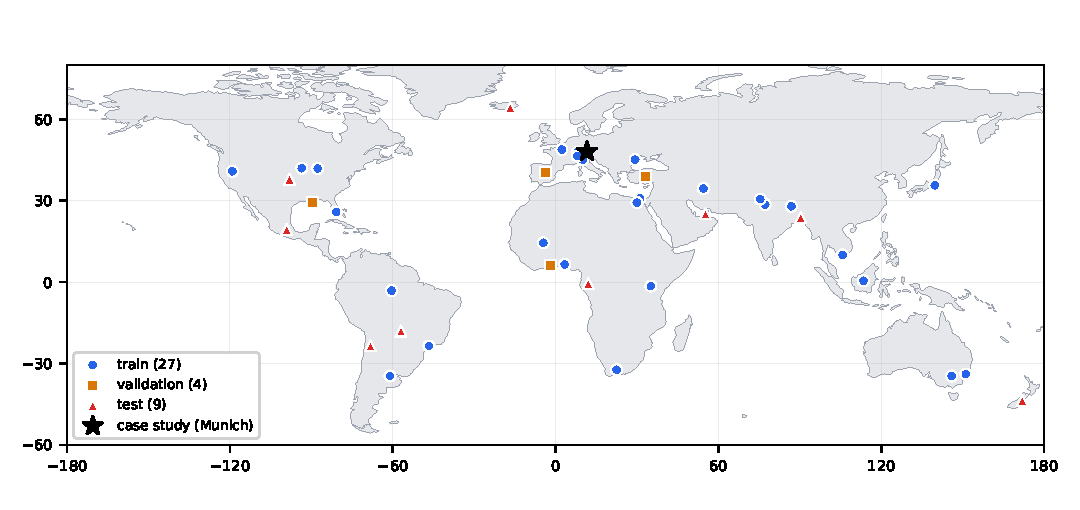
\includegraphics[width=\columnwidth]{figures/study_areas.pdf}
\caption{The 40 study areas. Training, validation and test areas are disjoint; the Munich case study lies outside
all of them (nearest study area 260\,km away).}
\label{fig:areas}
\end{figure}

\begin{table}[t]
\caption{Data splits (every second month, offset per year so that all calendar months occur)}
\label{tab:splits}
\centering\footnotesize
\setlength{\tabcolsep}{4pt}
\begin{tabular}{@{}llllr@{}}
\toprule
Split & Regions & Areas & Period (months) & Patches \\
\midrule
Training & train & 26$^{*}$ & 2023--24 (12) & 14\,952 \\
Validation & val & 4 & 2023--24 (12) & 1\,808 \\
Test & unseen & 9 & 2025--26 (11) & 4\,536 \\
Test temporal & train & 26 & 2025--26 (6) & 7\,041 \\
\bottomrule
\multicolumn{5}{@{}l}{\scriptsize $^{*}$27 planned; Everest lost to the Earth Engine quota (Section~III-D).}
\end{tabular}
\end{table}

\subsection{Sentinel-1 input and preprocessing}

The input is the Sentinel-1 ground-range-detected collection of Earth Engine (\texttt{COPERNICUS/S1\_GRD}; IW mode,
VV and VH, 10\,m). In this
collection every scene is already processed with the ESA Sentinel-1 toolbox: orbit-file correction, GRD border-noise
removal, thermal-noise removal, radiometric calibration to $\sigma^0$, terrain correction with the SRTM 30\,m
elevation model (ASTER above 60$^\circ$ latitude) and conversion to decibels. On top of that, the following steps were applied (Table~\ref{tab:prep}):

\textit{Orbit pass.} Backscatter depends on look direction and incidence angle, so ascending and descending scenes of
the same place differ. Each study area uses only the pass with more scenes in its period; mixing passes would create
apparent month-to-month change.

\textit{Residual border noise and speckle.} Pixels with VV below $-30$\,dB are masked as residual border
noise or no-return areas. Each scene is filtered in linear power
with the Lee filter~\cite{lee1980digital},
\begin{equation}
\hat{x}=\bar{x}+W\,(x-\bar{x}),\quad W=\mathrm{clip}_{[0,1]}\!\left(\frac{1-C_u^2/C_I^2}{1+C_u^2}\right),
\end{equation}
with a $5\times5$ window, $C_u^2=1/\mathrm{ENL}$ (ENL\,$=4.4$ for IW GRD) and $C_I^2=\mathrm{Var}(x)/\bar{x}^2$.

\textit{Monthly compositing.} The per-pixel median of all filtered scenes in a month forms the composite, which also
acts as temporal multi-looking. It is converted back to dB, and the VV$-$VH difference is added as a third channel.

\begin{table}[t]
\caption{Preprocessing chain}
\label{tab:prep}
\centering\footnotesize
\begin{tabular}{@{}p{2.3cm}p{5.6cm}@{}}
\toprule
Step & Implementation \\
\midrule
Calibration, terrain correction, dB & Earth Engine S1\_GRD: orbit file, border and thermal noise removal, $\sigma^0$, SRTM/ASTER terrain correction \\
Scene selection & IW, VV+VH, 10\,m, one orbit pass per area \\
Border noise & VV $<-30$\,dB masked \\
Speckle filter & Lee, $5\times5$, ENL 4.4, linear power, per scene \\
Compositing & monthly per-pixel median; VV, VH, VV$-$VH in dB \\
Label matching & Dynamic World, same month and grid: mean class probability $\rightarrow$ argmax \\
Label quality & top-class probability $<0.3$ or no observation $\rightarrow$ ignored \\
Patching & $256\times256$, non-overlapping; drop patches with S1 gaps or $<50$\,\% labels \\
Normalisation & clip VV $[-25,0]$, VH $[-32,-5]$, VV$-$VH $[-5,20]$\,dB; z-score (training statistics) \\
Augmentation & flips, $90^\circ$ rotations, $\pm1$\,dB brightness (VV and VH jointly), speckle noise $\sigma=0.3$\,dB \\
\bottomrule
\end{tabular}
\end{table}

\subsection{Labels and their matching to the imagery}

Labels come from Dynamic World V1~\cite{brown2022dynamic}, which provides per-image class probabilities for nine
classes from Sentinel-2. For each area and month the probabilities of all cloud-free observations were averaged and
the most probable class was taken, on exactly the same 10\,m grid as the radar composite, so image and label refer to
the same month and footprint. Pixels whose mean top-class probability is below 0.3, or that had no cloud-free
observation, are set to an ignore index. In a preliminary dataset of German study areas, a threshold of 0.5 had removed almost all
grassland and bare-ground pixels (0.7\,\% and 0.05\,\% of the labels remained), so 0.3 was used. Grass and shrub/scrub were merged into \emph{rangeland}, which gives eight classes identical to the
Esri map without its cloud class (Table~\ref{tab:classes}); this choice allows a class-by-class comparison with that
independent map in the case study.

\begin{table}[t]
\caption{Classes and pixel distribution (\% of labelled pixels)}
\label{tab:classes}
\centering\footnotesize
\setlength{\tabcolsep}{3.5pt}
\begin{tabular}{@{}lrrrrr@{}}
\toprule
Class & Train & Val & Test & Test temp. & Loss $w_c$ \\
\midrule
Water & 9.10 & 16.05 & 5.20 & 9.83 & 1.30 \\
Trees & 11.49 & 12.73 & 13.97 & 11.82 & 1.03 \\
Flooded vegetation & 2.85 & 2.54 & 0.08 & 1.55 & 4.14 \\
Crops & 20.26 & 23.86 & 12.88 & 20.05 & 0.58 \\
Rangeland$^{*}$ & 12.12 & 4.36 & 11.08 & 12.97 & 0.97 \\
Built-up & 23.65 & 24.70 & 24.20 & 23.37 & 0.50 \\
Bare & 17.97 & 15.74 & 19.06 & 17.51 & 0.66 \\
Snow/ice & 2.56 & 0.02 & 13.54 & 2.90 & 4.62 \\
\bottomrule
\multicolumn{6}{@{}l}{\scriptsize $^{*}$Dynamic World grass and shrub/scrub merged.}
\end{tabular}
\end{table}

\subsection{Dataset}

The export downloaded, for each area-month, four $1024\times1024$ tiles with six bands (VV, VH, VV$-$VH, Dynamic World
class, confidence, number of observations) through Earth Engine's \texttt{computePixels} interface. In the final
export run over all 633 area-months, 511 were complete, 40 were skipped because no Sentinel-1 scene or no cloud-free
label existed (e.g., Amazon and Lagos in cloudy months), and 82 could not be completed after the project had used up
its monthly noncommercial quota. This removed all months of the Everest area, so snow/ice in training comes only from
the Aletsch glacier, whereas the test set contains a large glacier (Vatnajökull). In total 2\,265 tiles were
downloaded and cut into the patches of Table~\ref{tab:splits}. The dataset is
available on Kaggle (see Data Availability).

% =====================================================================================================
\section{Methods}

\subsection{Models}

Three architectures of increasing capacity were compared first (Table~\ref{tab:models}): a \emph{baseline CNN} of four
$3\times3$ convolutions at full resolution (receptive field 90\,m), which tests how much backscatter and local texture
alone explain; a \emph{U-Net}~\cite{ronneberger2015unet} trained from scratch with four down-sampling stages
(receptive field of about 2\,km) and spatial dropout; and \emph{DeepLabV3+}~\cite{chen2018encoder} with an
ImageNet-pretrained ResNet50 cut after the 1/16-resolution stage, ASPP (rates 6, 12, 18 plus image pooling) and a
decoder fusing 1/4-resolution features. The three SAR channels replace RGB; low-level pretrained filters transfer and
are fine-tuned.

Six DeepLabV3+ variants then tested the encoder: ResNet101, ResNet152 and Xception, each in the standard cut-off form
and as an \emph{atrous encoder} (AE) that keeps the full backbone but replaces the stride of its last stage by dilation
2, so that features stay at output stride 16 as in the original DeepLab design~\cite{chen2017rethinking}. Finally, a
\emph{multi-temporal} DeepLabV3+ with ResNet50 receives the target month and the two previous exported months (2--3
months apart) as nine channels; its first-layer filters are the pretrained filters copied to every month and divided
by three, so that three identical months reproduce the single-month response.

\begin{table*}[t]
\caption{Model overview}
\label{tab:models}
\centering\small
\begin{tabular}{@{}llrlrr@{}}
\toprule
Model & Input & Params & Encoder & LR & Batch \\
\midrule
Baseline CNN & 1 month & 0.08\,M & -- (4 conv layers) & $10^{-3}$ & 16 \\
U-Net & 1 month & 7.9\,M & from scratch & $10^{-3}$ & 16 \\
DeepLabV3+ & 1 month & 11.9\,M & ResNet50 (ImageNet), cut at 1/16 & $3\cdot10^{-4}$ & 16 \\
DeepLabV3+ (E1--E3) & 1 month & 24.6--52.6\,M & Xception, ResNet101, ResNet152 & $3\cdot10^{-4}$ & 8 \\
AE-DeepLabV3+ (E4--E6) & 1 month & 37.7--75.2\,M & same, full backbone, atrous last stage & $3\cdot10^{-4}$ & 8 \\
DeepLabV3+ (multi-temporal) & 3 months & 11.9\,M & ResNet50, first layer for 9 channels & $3\cdot10^{-4}$ & 16 \\
\bottomrule
\end{tabular}
\end{table*}

\subsection{Training}

\textit{Normalisation and augmentation.} Each channel is clipped to a fixed dB range and z-scored with the mean and
standard deviation of the training split only (Table~\ref{tab:prep}), and the same statistics are used at inference.
During training, patches are randomly flipped and rotated by multiples of $90^\circ$, because land cover has no
preferred orientation. In addition, the same random offset of up to $\pm1$\,dB is added to VV and VH, which leaves
their ratio unchanged and mimics calibration and incidence-angle differences between scenes, orbits and satellites
(Sentinel-1A in the training period, Sentinel-1A and 1C in the test period), and Gaussian noise with
$\sigma=0.3$\,dB imitates residual speckle. Larger or per-channel intensity changes were avoided because they would
alter the physical meaning of the backscatter, e.g., make water resemble vegetation.

\textit{Loss and optimisation.} All models minimise class-weighted cross-entropy plus soft Dice over labelled pixels $p$,
\begin{align}
\mathcal{L}&=\mathcal{L}_{\mathrm{CE}}+\mathcal{L}_{\mathrm{Dice}},\qquad
\mathcal{L}_{\mathrm{CE}}=-\frac{\sum_p w_{y_p}\log s_{p,y_p}}{\sum_p w_{y_p}},\\
\mathcal{L}_{\mathrm{Dice}}&=1-\frac{1}{K}\sum_{c=1}^{K}\frac{2\sum_p g_{pc}s_{pc}+1}{\sum_p (g_{pc}+s_{pc})+1},
\end{align}
where $s$ are softmax scores, $g$ one-hot labels and $w_c=\mathrm{clip}_{[0.2,10]}\big(\mathrm{median}(f)/f_c\big)$ the
median-frequency weights~\cite{eigen2015predicting} computed from the class frequencies $f_c$ (Table~\ref{tab:classes});
Dice~\cite{milletari2016vnet} measures overlap per class and is less dominated by frequent classes. Optimisation used
AdamW~\cite{loshchilov2019decoupled} (weight decay $10^{-4}$) with mixed precision on an NVIDIA RTX~A6000 in
TensorFlow~2.20. After every epoch, exact mIoU and overall accuracy were computed on the validation set and on 1\,000
fixed training patches. The learning rate was halved after 3 epochs without validation-mIoU improvement, training
stopped after 8 such epochs (at most 50) and the best epoch was kept. A model was labelled \emph{underfitting} if its
training mIoU at the best epoch was below 0.35 and \emph{overfitting} if training exceeded validation mIoU by more
than 0.15.

\subsection{Evaluation}

With confusion matrix $n_{ij}$ (reference $i$, prediction $j$) over $N$ labelled test pixels,
\begin{gather}
\mathrm{OA}=\frac{1}{N}\sum_c n_{cc},\qquad
\mathrm{IoU}_c=\frac{n_{cc}}{n_{c\cdot}+n_{\cdot c}-n_{cc}},\\
F1_c=\frac{2n_{cc}}{n_{c\cdot}+n_{\cdot c}},
\end{gather}
and mIoU and mean F1 average over classes present in the reference. Model selection used the validation mIoU only;
differences smaller than its epoch-to-epoch variation were treated as ties in favour of the simpler model.

% =====================================================================================================
\section{Results}

\subsection{Architecture comparison}

Table~\ref{tab:main} and Fig.~\ref{fig:curves} summarise the first comparison. Context and pretraining help: test mIoU
rises from 0.203 (baseline) to 0.275 (U-Net) and 0.304 (DeepLabV3+), which was selected on validation mIoU. The
baseline is weak even on training data (underfitting), whereas U-Net and DeepLabV3+ reach a training mIoU near 0.6 but
only about 0.4 on the validation regions (overfitting). Early stopping ended the runs after 18--25 epochs.

\begin{table*}[t]
\caption{Architecture comparison. Test: nine unseen regions, 2025--26. Test temporal: training regions, 2025--26}
\label{tab:main}
\centering\footnotesize
\begin{tabular}{@{}lrrrrrcrrrcrr@{}}
\toprule
& & & \multicolumn{3}{c}{mIoU at best epoch} && \multicolumn{3}{c}{Test} && \multicolumn{2}{c}{Test temporal} \\
\cmidrule{4-6}\cmidrule{8-10}\cmidrule{12-13}
Model & Epochs & Best & Train & Val & Gap && OA & mIoU & mF1 && OA & mIoU \\
\midrule
Baseline CNN & 18 & 10 & 0.337 & 0.306 & 0.031 && 0.420 & 0.203 & 0.303 && 0.557 & 0.332 \\
U-Net & 25 & 17 & 0.593 & 0.381 & 0.212 && 0.496 & 0.275 & 0.365 && \textbf{0.782} & \textbf{0.576} \\
DeepLabV3+ (ResNet50) & 24 & 16 & 0.619 & \textbf{0.399} & 0.220 && \textbf{0.510} & \textbf{0.304} & \textbf{0.402} && 0.755 & 0.565 \\
\bottomrule
\end{tabular}
\end{table*}

\begin{figure*}[t]
\centering
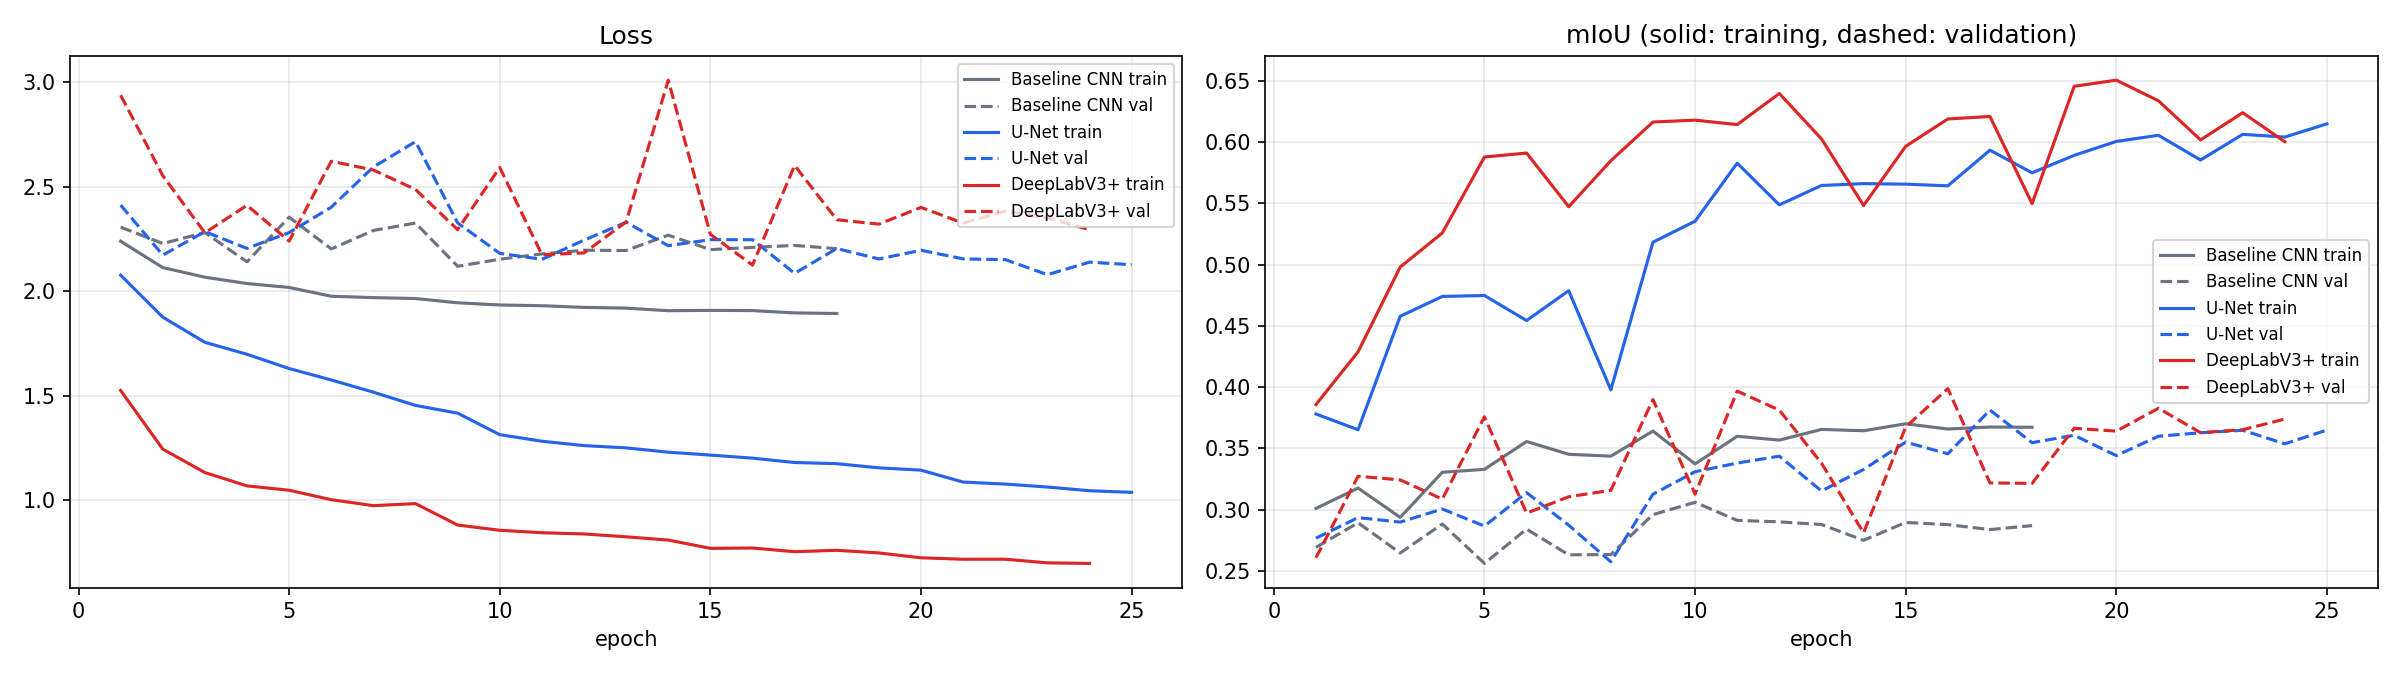
\includegraphics[width=0.92\textwidth]{figures/training_curves.png}
\caption{Training curves of the three architectures (solid: training, dashed: validation). Validation mIoU fluctuates
by up to $\pm0.08$ between epochs because the four validation regions differ strongly.}
\label{fig:curves}
\end{figure*}

\subsection{Generalisation to new regions and dates}

On the training regions in 2025--26, U-Net and DeepLabV3+ reach OA 0.76--0.78 and mIoU 0.56--0.58 (Table~\ref{tab:main}),
against 0.50--0.51 and 0.27--0.30 on the unseen test regions. The models therefore cope well with a later period but
much less with new landscapes: the overfitting is geographic. Per region (Table~\ref{tab:regions}), Gabon, Mexico City,
Pantanal and Dhaka are classified with OA 0.74--0.97, while Atacama (salt flats, OA 0.03) and Vatnajökull (glacier,
OA 0.00) fail almost completely. The confusion matrix (Fig.~\ref{fig:cm}) explains the failure: 66\,\% of the bare
pixels are predicted as snow/ice and 40\,\% of the snow/ice pixels as water. Crops and rangeland are confused in both
directions (22\,\% and 27\,\%), and flooded vegetation is mostly predicted as trees or water. Built-up (IoU 0.78),
trees (0.54) and water (0.36) are the most reliable classes (Table~\ref{tab:perclass}).

\begin{table}[t]
\caption{DeepLabV3+ (ResNet50) per test region}
\label{tab:regions}
\centering\footnotesize
\begin{tabular}{@{}lrrr@{}}
\toprule
Region (landscape) & OA & mIoU & Patches \\
\midrule
Gabon (forest) & 0.973 & 0.139 & 84 \\
Mexico City (urban) & 0.868 & 0.199 & 593 \\
Pantanal (wetland) & 0.770 & 0.160 & 642 \\
Dhaka (urban) & 0.742 & 0.262 & 359 \\
Dubai (urban, desert) & 0.650 & 0.198 & 574 \\
Kansas (cropland) & 0.605 & 0.283 & 615 \\
Canterbury NZ (cropland) & 0.452 & 0.144 & 509 \\
Atacama (salt flats) & 0.027 & 0.004 & 641 \\
Vatnajökull (glacier) & 0.004 & 0.004 & 519 \\
\bottomrule
\end{tabular}
\end{table}

\begin{figure}[t]
\centering
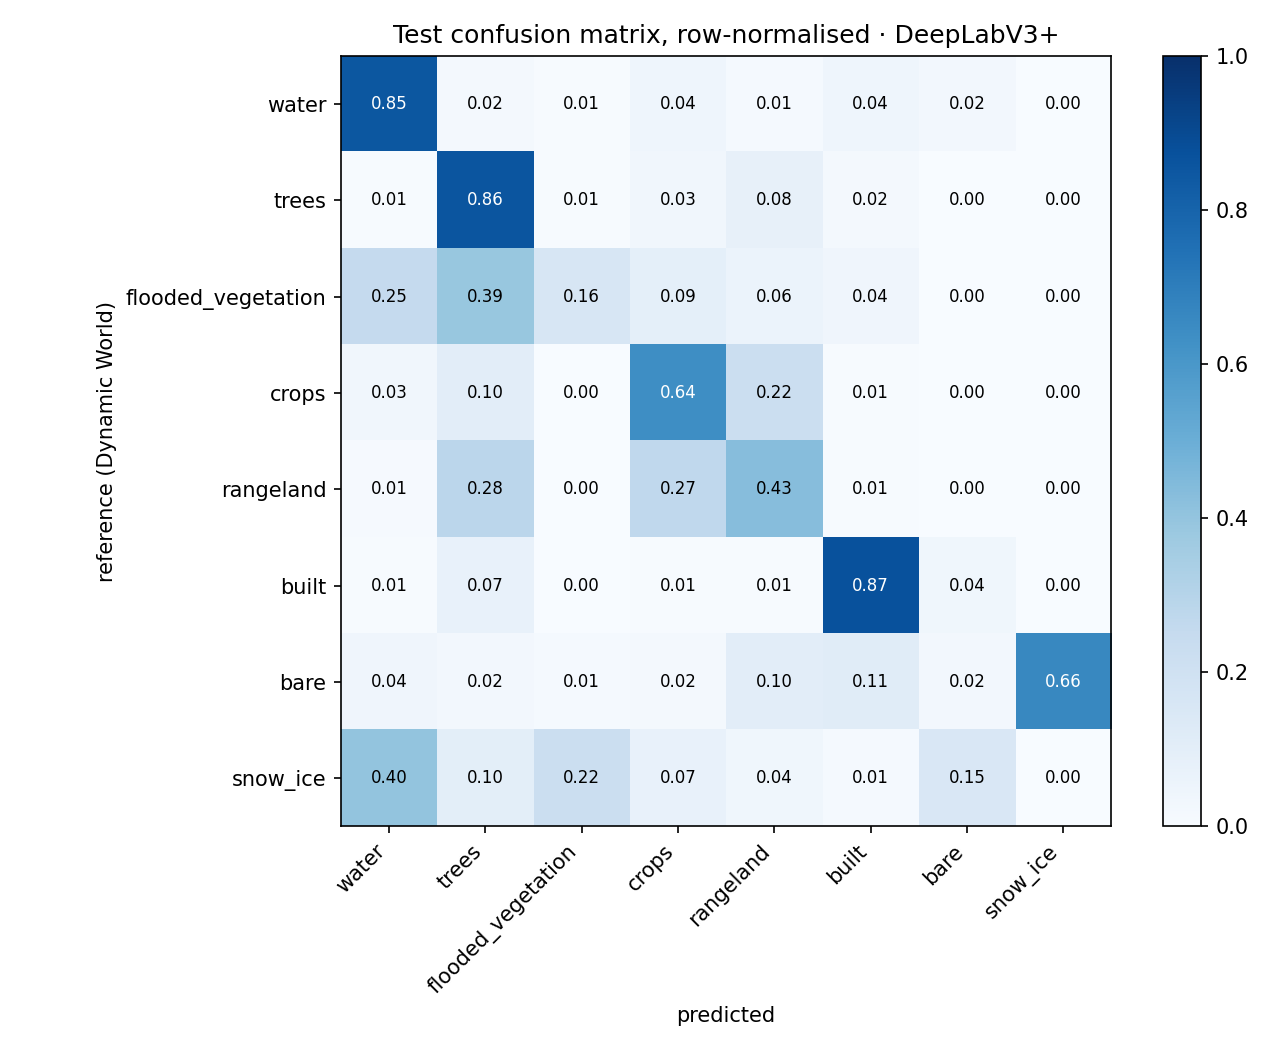
\includegraphics[width=0.95\columnwidth]{figures/confusion_matrix.png}
\caption{Row-normalised test confusion matrix of DeepLabV3+ (ResNet50).}
\label{fig:cm}
\end{figure}

\begin{table}[t]
\caption{Test IoU / F1 per class}
\label{tab:perclass}
\centering\footnotesize
\begin{tabular}{@{}lccc@{}}
\toprule
Class & Baseline & U-Net & DeepLabV3+ \\
\midrule
Water & 0.28 / 0.44 & 0.33 / 0.50 & \textbf{0.36} / \textbf{0.53} \\
Trees & 0.34 / 0.51 & 0.33 / 0.50 & \textbf{0.54} / \textbf{0.70} \\
Flooded veg. & 0.01 / 0.01 & 0.00 / 0.00 & 0.00 / 0.01 \\
Crops & 0.21 / 0.34 & \textbf{0.51} / \textbf{0.67} & 0.46 / 0.63 \\
Rangeland & \textbf{0.27} / \textbf{0.42} & 0.18 / 0.30 & \textbf{0.27} / \textbf{0.42} \\
Built-up & 0.52 / 0.68 & \textbf{0.82} / \textbf{0.90} & 0.78 / 0.88 \\
Bare & 0.01 / 0.02 & 0.01 / 0.02 & 0.02 / 0.04 \\
Snow/ice & 0.00 / 0.00 & 0.01 / 0.03 & 0.00 / 0.00 \\
\bottomrule
\end{tabular}
\end{table}

\subsection{Encoder experiments}

Because both deep models overfit, the encoder was varied in a controlled experiment with otherwise identical settings
(Table~\ref{tab:exp}, Fig.~\ref{fig:exp}). Deeper encoders fit the training regions better without generalising better:
ResNet152 has the best validation mIoU (0.410) but a test mIoU of only 0.257. Xception overfits least (gap 0.14) but
also learns least. The atrous encoder lowers the validation mIoU but raises the test mIoU for all three backbones
(+0.008, +0.042, +0.025) and is the only change that lifts snow/ice above zero (IoU 0.10 for AE-ResNet152). None of the
six models with 25--75\,M parameters exceeds the 11.9\,M-parameter ResNet50 (0.304), and validation and test rankings
disagree. With four validation regions, a single region can decide the ranking, so the validation lead of ResNet152
(+0.011) was treated as a tie and the simpler ResNet50 was kept.

\begin{table*}[t]
\caption{Encoder experiments (batch 8). Gap = train $-$ val mIoU}
\label{tab:exp}
\centering\small
\begin{tabular}{@{}lrrrrrr@{}}
\toprule
DeepLabV3+ encoder & Parameters & Train mIoU & Val mIoU & Gap & Test OA & Test mIoU \\
\midrule
E1 Xception & 24.6\,M & 0.528 & 0.387 & 0.140 & 0.431 & 0.245 \\
E2 ResNet101 & 36.9\,M & 0.626 & 0.406 & 0.221 & 0.496 & 0.289 \\
E3 ResNet152 & 52.6\,M & 0.616 & \textbf{0.410} & 0.206 & 0.468 & 0.257 \\
E4 AE Xception & 37.7\,M & 0.593 & 0.383 & 0.211 & 0.487 & 0.270 \\
E5 AE ResNet101 & 59.5\,M & 0.579 & 0.356 & 0.223 & 0.511 & 0.297 \\
E6 AE ResNet152 & 75.2\,M & 0.614 & 0.357 & 0.257 & \textbf{0.518} & \textbf{0.299} \\
\midrule
Reference: ResNet50 (batch 16) & 11.9\,M & 0.619 & 0.399 & 0.220 & 0.510 & 0.304 \\
\bottomrule
\end{tabular}
\end{table*}

\begin{figure*}[t]
\centering
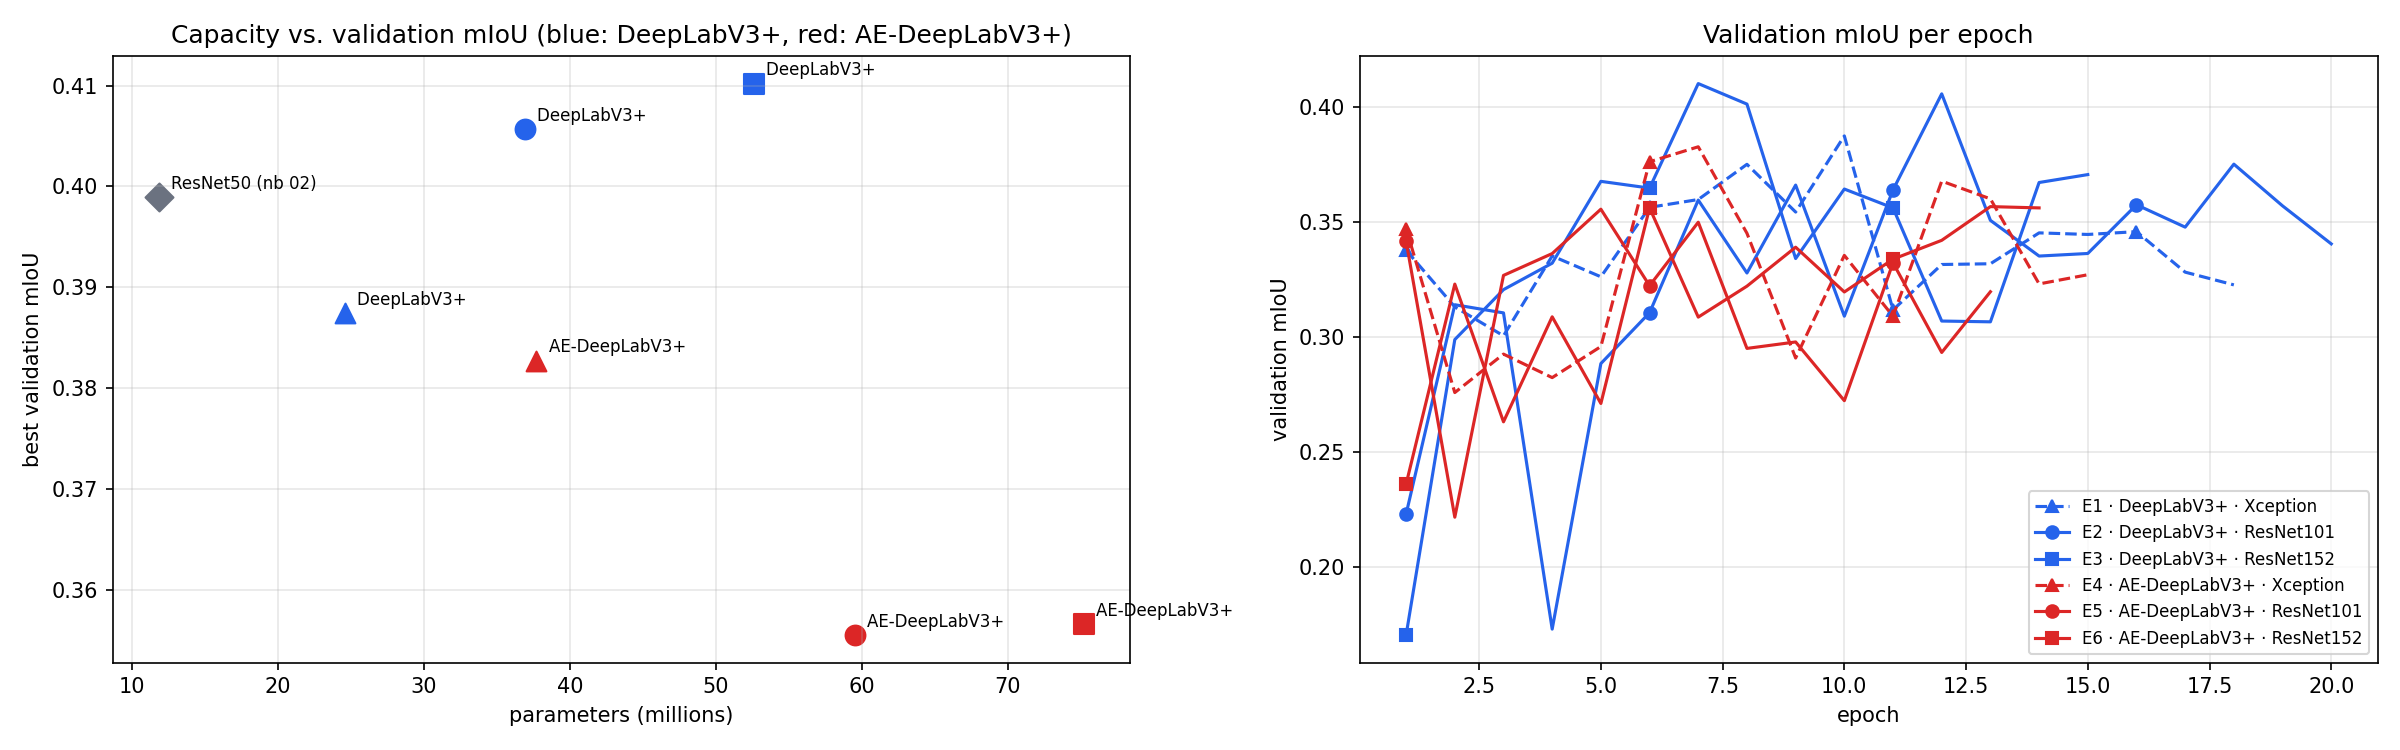
\includegraphics[width=0.92\textwidth]{figures/experiments_comparison.png}
\caption{Encoder experiments: capacity versus best validation mIoU (left) and validation mIoU per epoch (right).
Blue: DeepLabV3+, red: AE-DeepLabV3+.}
\label{fig:exp}
\end{figure*}

\subsection{Multi-temporal input}

The remaining confusions concern classes that differ mainly in their seasonal behaviour, so the third step changed
only the input to three months. Both models were evaluated on the same patches that have two earlier months
(Table~\ref{tab:mt}); this reduces the data to 11\,283 training, 810 validation and 2\,814 test patches. Temporal
information helps exactly where expected: cropland IoU rises from 0.552 to 0.646 and the two cropland test regions
improve (Kansas $+7.9$\pp~OA, Canterbury $+4.5$\pp). Overall, however, the model overfits more (gap 0.36 against
0.22), trees ($-0.195$ IoU), rangeland ($-0.115$) and the Pantanal wetland ($-8.6$\pp~OA) get worse, and the test
mIoU falls from 0.313 to 0.276. With three times more information per pixel, the network learns the seasonal rhythm of
the training regions, which does not transfer to other climates and hemispheres; only the crop cycle is similar
enough. The validation difference of $+0.005$ is again within the noise, so the single-month model remains the
prototype model.

\begin{table}[t]
\caption{Single-month vs. three-month input on the same patches}
\label{tab:mt}
\centering\footnotesize
\begin{tabular}{@{}lrrrrrr@{}}
\toprule
& \multicolumn{2}{c}{Validation} & \multicolumn{2}{c}{Test} & \multicolumn{2}{c}{Test IoU} \\
\cmidrule(lr){2-3}\cmidrule(lr){4-5}\cmidrule(l){6-7}
Input & OA & mIoU & OA & mIoU & crops & trees \\
\midrule
1 month & 0.615 & 0.344 & \textbf{0.487} & \textbf{0.313} & 0.552 & \textbf{0.517} \\
3 months & \textbf{0.637} & \textbf{0.348} & 0.480 & 0.276 & \textbf{0.646} & 0.322 \\
\bottomrule
\end{tabular}
\end{table}

\subsection{Radar-separable class scheme}

All ten models end near the same test mIoU, and their errors concentrate in the two class pairs identified above.
These pairs are easy to separate in optical imagery, from which the eight classes originate, but not in C-band
backscatter: dry snow is nearly transparent~\cite{nagler2000retrieval,ulaby2014microwave} and resembles the ground beneath, and fields,
grassland and shrubland have similar roughness and moisture in a single month. The predictions of the prototype model
were therefore re-evaluated, without retraining, after merging crops and rangeland into \emph{low vegetation} and bare
and snow/ice into \emph{bare/snow} (Table~\ref{tab:scheme}, Fig.~\ref{fig:cm6}). The overall accuracy rises from 0.510
to 0.715 and the mIoU from 0.304 to 0.461; bare/snow reaches IoU 0.45 (previously 0.02 and 0.00) and low vegetation
0.63. Without the two extreme test regions, the six-class OA is 0.772, close to the 0.76--0.78 reached on the training
regions. Flooded vegetation, with only 0.08\,\% of the test pixels, stays near zero but counts as a full class in the
mean; the other five classes average an IoU of about 0.55.

\begin{table}[t]
\caption{Same predictions (prototype model) under two class schemes}
\label{tab:scheme}
\centering\footnotesize
\setlength{\tabcolsep}{4pt}
\begin{tabular}{@{}llrrr@{}}
\toprule
Test regions & Classes & OA & mIoU & mF1 \\
\midrule
All nine & 8 (original) & 0.510 & 0.304 & 0.402 \\
& 6 (merged) & \textbf{0.715} & \textbf{0.461} & \textbf{0.585} \\
\midrule
Without the & 8 (original) & 0.692 & 0.355 & 0.454 \\
two extremes$^{*}$ & 6 (merged) & \textbf{0.772} & 0.459 & 0.556 \\
\bottomrule
\multicolumn{5}{@{}l}{\scriptsize $^{*}$Atacama (salt flats) and Vatnajökull (glacier).}
\end{tabular}
\end{table}

\begin{figure}[t]
\centering
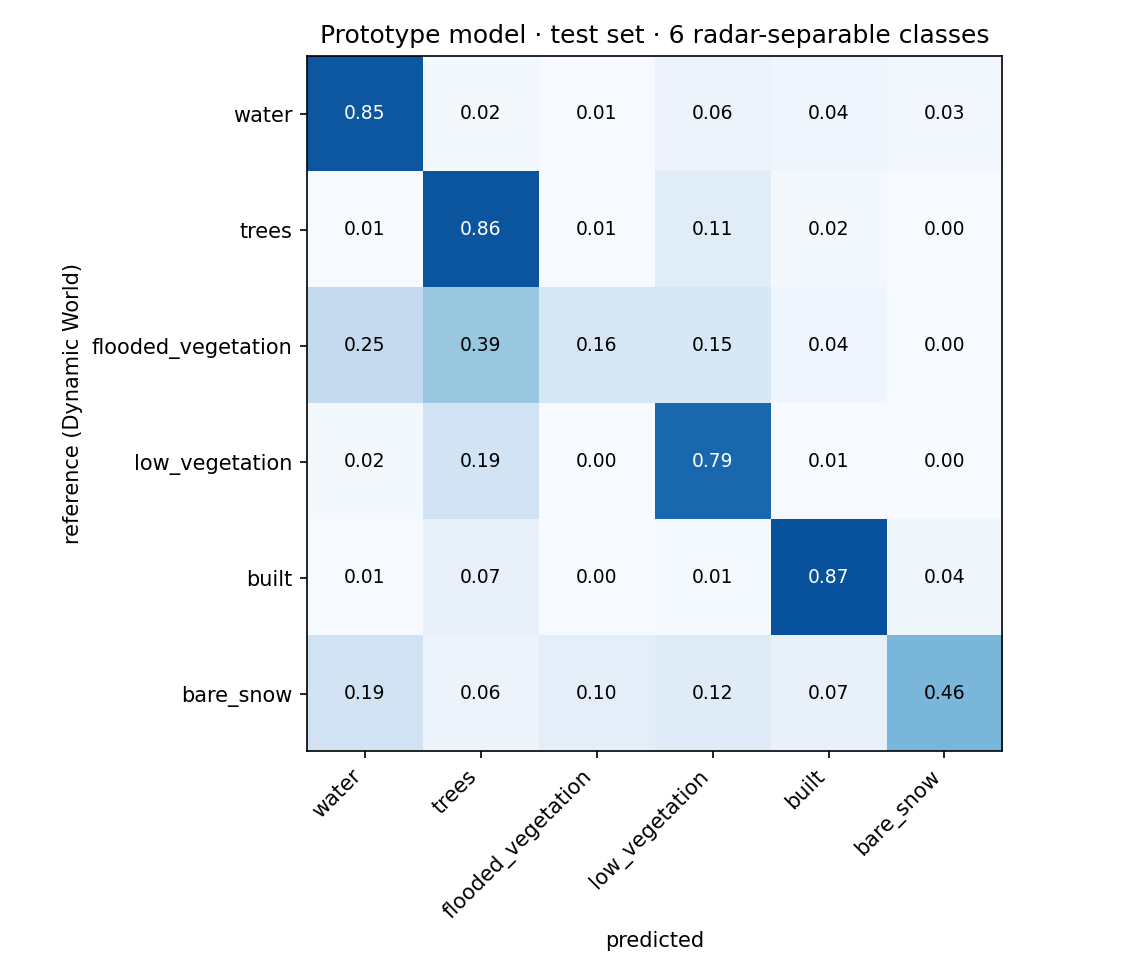
\includegraphics[width=0.85\columnwidth]{figures/confusion_6_classes.png}
\caption{Test confusion matrix of the prototype model in the six-class scheme.}
\label{fig:cm6}
\end{figure}

% =====================================================================================================
\section{Prototype}

\subsection{System architecture}

The prototype (Fig.~\ref{fig:arch}) is a Streamlit web application on top of a Python package that is shared with the
training code, so that inference uses exactly the training preprocessing. The user enters a place name (resolved
through OpenStreetMap Nominatim, with a choice among up to five matches) or coordinates, a start month and an area of
2.56, 5.12 or 10.24\,km. A run takes about 30--90\,s on a laptop CPU.

\begin{figure}[t]
\centering
\resizebox{\columnwidth}{!}{%
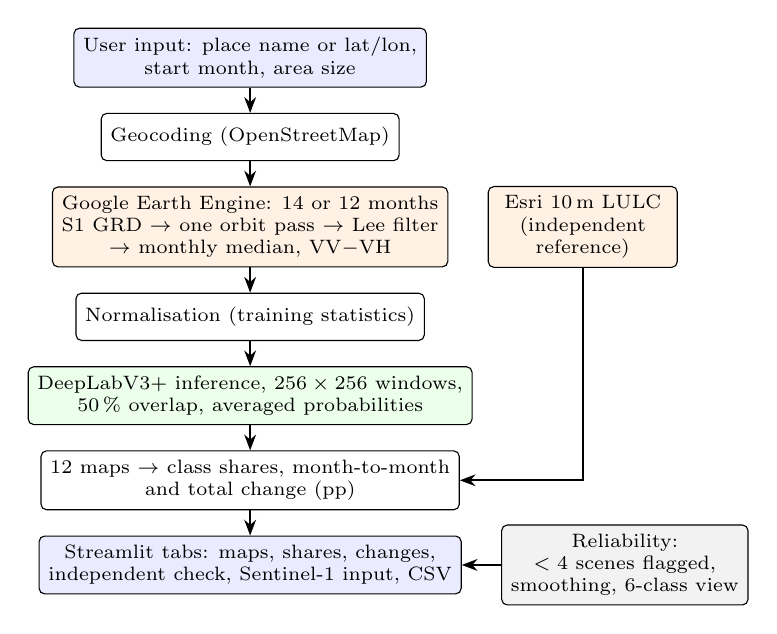
\begin{tikzpicture}[node distance=3.2mm, font=\scriptsize,
  box/.style={draw, rounded corners=2pt, align=center, minimum width=3.6cm, minimum height=6mm, fill=#1},
  box/.default=white, arr/.style={-{Stealth[length=2mm]}, semithick}]
\node[box=blue!8] (in) {User input: place name or lat/lon,\\ start month, area size};
\node[box, below=of in] (geo) {Geocoding (OpenStreetMap)};
\node[box=orange!10, below=of geo] (gee) {Google Earth Engine: 14 or 12 months\\ S1 GRD $\rightarrow$ one orbit pass $\rightarrow$
Lee filter\\ $\rightarrow$ monthly median, VV$-$VH};
\node[box, below=of gee] (norm) {Normalisation (training statistics)};
\node[box=green!8, below=of norm] (net) {DeepLabV3+ inference, $256\times256$ windows,\\ 50\,\% overlap, averaged probabilities};
\node[box, below=of net] (stat) {12 maps $\rightarrow$ class shares, month-to-month\\ and total change (pp)};
\node[box=blue!8, below=of stat] (ui) {Streamlit tabs: maps, shares, changes,\\ independent check, Sentinel-1 input, CSV};
\node[box=orange!10, right=5mm of gee, minimum width=2.4cm] (esri) {Esri 10\,m LULC\\ (independent\\ reference)};
\node[box=gray!10, right=5mm of ui, minimum width=2.4cm] (rel) {Reliability:\\ $<4$ scenes flagged,\\ smoothing, 6-class view};
\foreach \a/\b in {in/geo, geo/gee, gee/norm, norm/net, net/stat, stat/ui} \draw[arr] (\a) -- (\b);
\draw[arr] (esri) |- (stat.east); \draw[arr] (rel) -- (ui);
\end{tikzpicture}}
\caption{Prototype architecture.}
\label{fig:arch}
\end{figure}

\subsection{Data retrieval and monthly compositing}

For the selected square, Earth Engine selects the orbit pass with more scenes over the whole twelve months and uses it
for every month, then builds each monthly composite with the training chain (Table~\ref{tab:prep}); a model with
temporal input additionally receives the earlier months. Composites are requested on the exact 10\,m UTM grid with
\texttt{computePixels}, so no export or storage is needed. Months without any scene are shown as empty and excluded
from the statistics, and months composited from fewer than four scenes are flagged because they retain more speckle and
are dominated by single acquisitions.

\subsection{Class percentages and changes}

For month $m$ with valid (radar-covered) pixels $V(m)$ and predicted class $\hat{y}_p(m)$, the class share and the
changes in percentage points are
\begin{align}
s_c(m)&=100\cdot\frac{|\{p\in V(m):\hat{y}_p(m)=c\}|}{|V(m)|},\\
\Delta_c(m)&=s_c(m)-s_c(m-1),\\
\Delta_c^{\mathrm{tot}}&=s_c(m_{12})-s_c(m_1).
\end{align}
Two optional views help to judge the result: a three-month majority filter per pixel that suppresses one-month
flicker, and the six-class scheme of Table~\ref{tab:scheme}. For the independent check, the most frequent class per
pixel over the twelve months is compared with the Esri 10\,m Annual LULC map~\cite{karra2021global}, which is produced
from Sentinel-2 by a different model and was not used in training.

\subsection{Case study: Munich, 2025}

Munich (10.24\,km around the city centre, January--December 2025, 7--14 descending scenes per month) lies 260\,km
from the nearest study area. The twelve maps (Fig.~\ref{fig:munich}) reproduce the Isar, the Englischer Garten and the
riverside forests. The pixel agreement with Esri~2025 is 87.9\,\%; built-up, which covers 92\,\% of the area, reaches
F1 0.94 against Esri (Fig.~\ref{fig:esri}). The largest difference is trees (model 14.9\,\%, Esri 4.6\,\%), largely a
difference of definitions: Esri maps trees inside the city as built area, whereas Dynamic World, the training reference,
maps them as trees. In the six-class scheme the agreement is 88.1\,\%; the merged classes cover only 1--2\,\% of
Munich, so the large gain of Table~\ref{tab:scheme} comes from cropland, steppe, desert and glacier landscapes.

The monthly shares (Fig.~\ref{fig:shares}) show a seasonal cycle without real land-use change: trees rise from
10.6\,\% in January to 17.1\,\% in July and built-up falls from 86.7\,\% to 81.1\,\%, because leafless trees produce
little volume scattering. The total change January$\to$December is $+5.3$\pp~trees and $-4.5$\pp~built-up, which would
correspond to 4.7\,km$^2$ of lost built-up area. One genuine temporary change is captured: a large smooth square, most
likely the Theresienwiese, appears as water from January to June (specular reflection) and as built-up from July to
November, when the Oktoberfest structures are put up, used and removed.

\begin{figure*}[t]
\centering
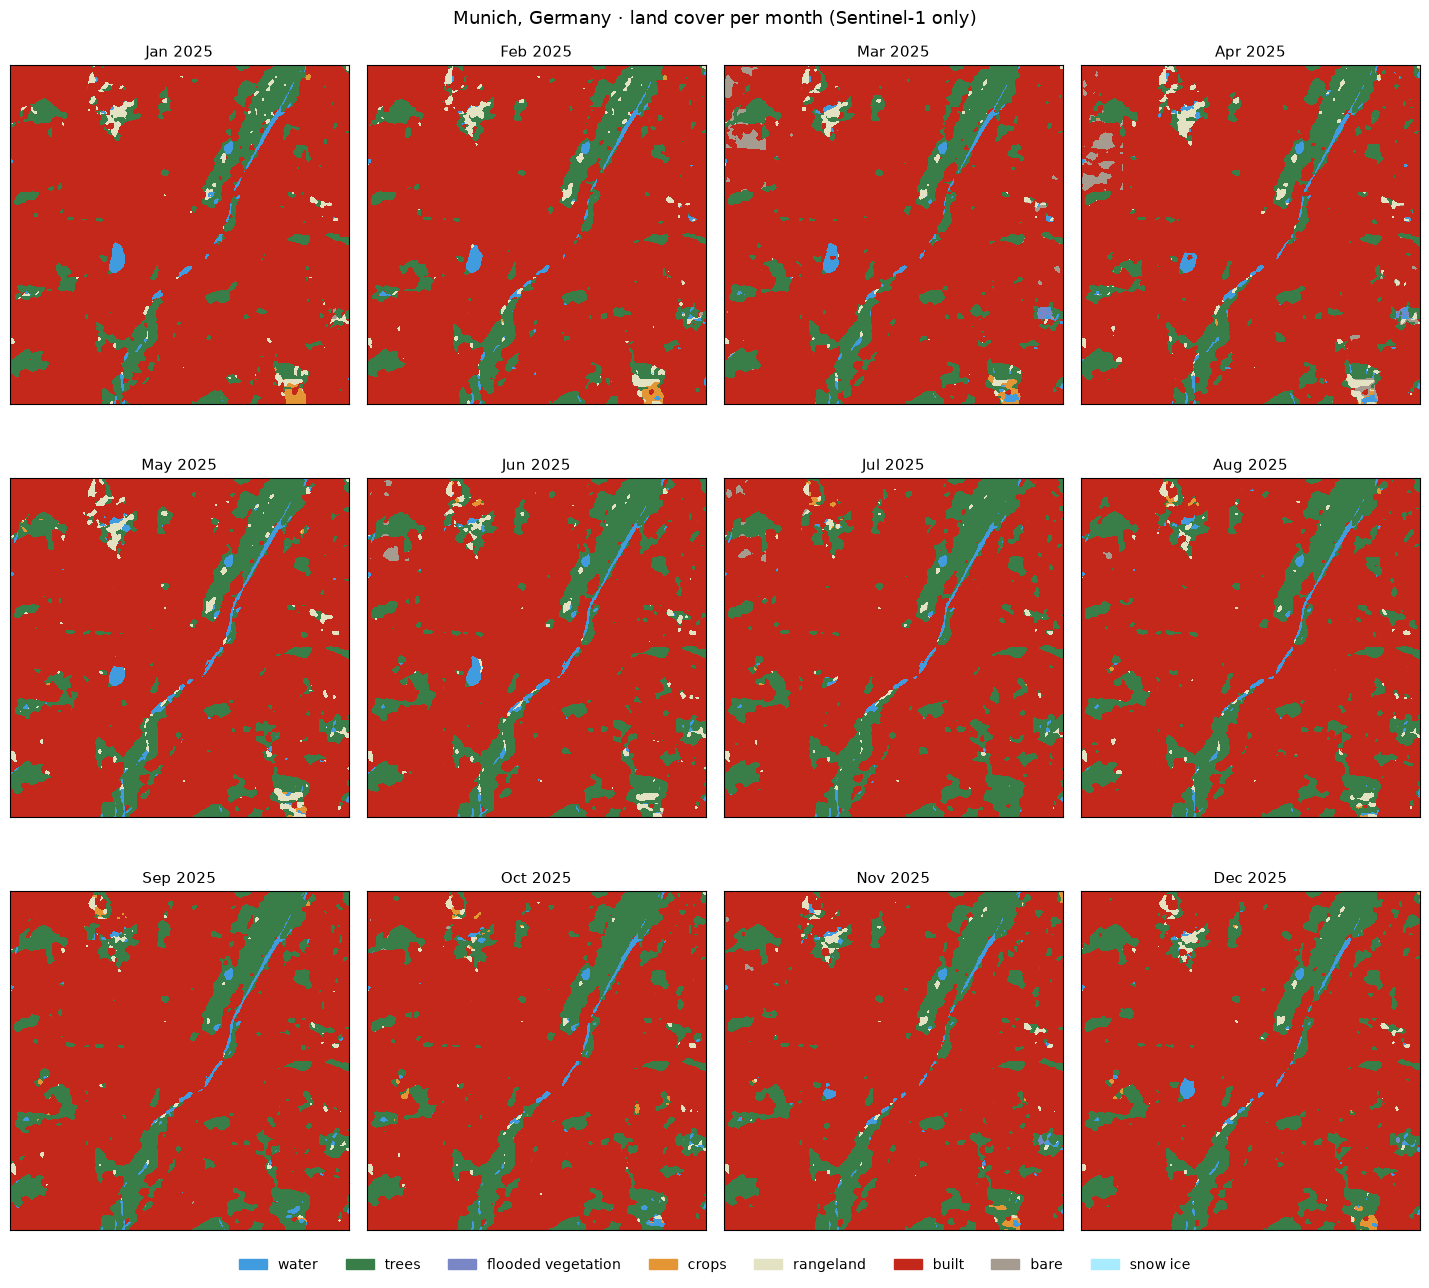
\includegraphics[width=0.9\textwidth]{figures/04_cell4_0.png}
\caption{Case study Munich: twelve monthly land-cover maps (2025) from Sentinel-1 only.}
\label{fig:munich}
\end{figure*}

\begin{figure}[t]
\centering
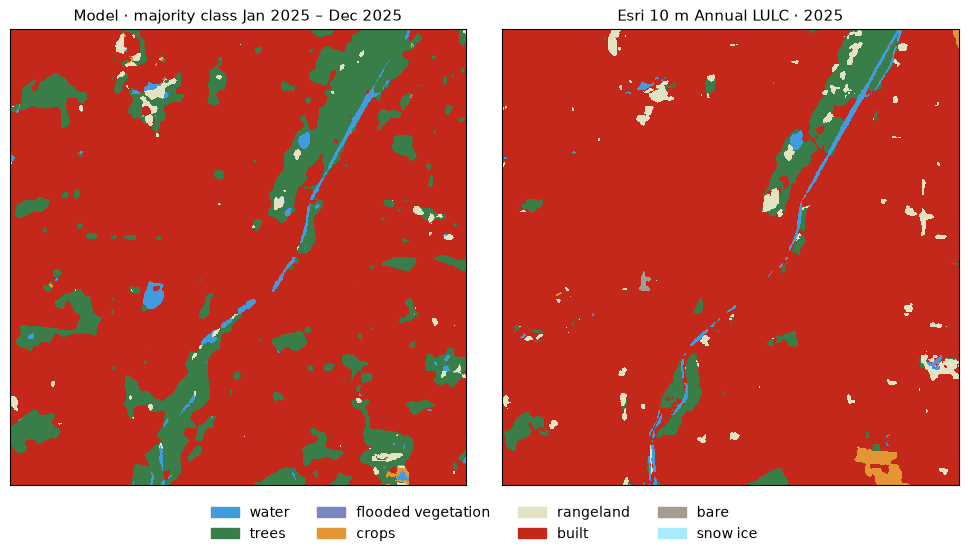
\includegraphics[width=\columnwidth]{figures/04_cell10_0.png}
\caption{Munich: majority class over 2025 (left) and the independent Esri 10\,m Annual LULC map 2025 (right).}
\label{fig:esri}
\end{figure}

\begin{figure}[t]
\centering
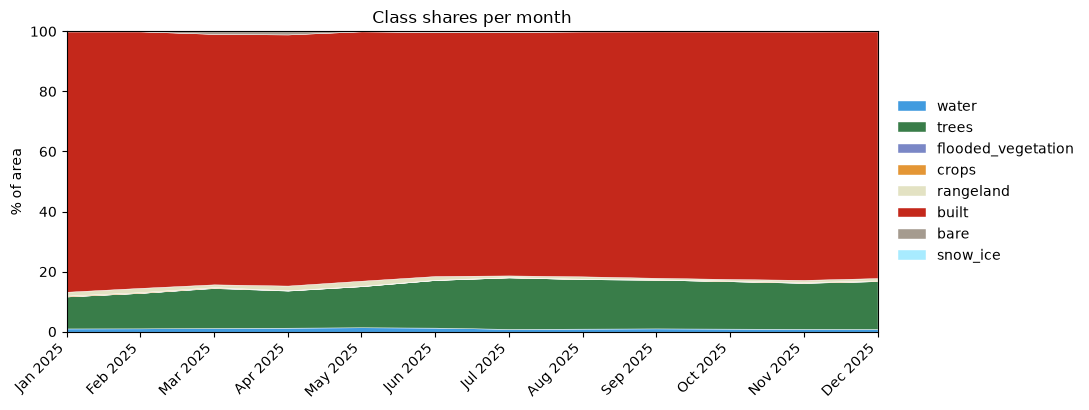
\includegraphics[width=\columnwidth]{figures/04_cell6_0.png}
\caption{Munich: class shares per month. The tree share follows the leaf-on/leaf-off cycle.}
\label{fig:shares}
\end{figure}

% =====================================================================================================
\section{Discussion}

\subsection{Regions unlike the training data}

The gap between familiar regions (mIoU 0.56--0.58) and unseen regions (about 0.30) is the dominant error source, and
neither larger encoders nor temporal input reduced it. Landscapes absent from training fail: the hyper-arid Atacama
salt flats and the Vatnajökull ice cap. The quota-related loss of the Everest area made this worse by leaving a single
glacier in training. The prototype shows the same effect for Kampala, where no East African city exists in training.
Training on many more climates, and validation with more regions or region-wise cross-validation, would address both
generalisation and the unstable model selection observed here.

\subsection{SAR-specific confusion}

Bare ground and snow/ice, cropland and rangeland, and smooth paved surfaces and water are confused because their
C-band backscatter is similar; flooded vegetation is labelled as trees or water depending on whether canopy or open
water dominates the signal. These are physical limits of a single-frequency, dual-polarisation sensor rather than
deficits of a particular network, which is why the radar-separable scheme improves the accuracy so strongly. A
Sentinel-1-only product should report such merged classes, or at least communicate the expected confusions.

\subsection{Seasonal effects that resemble land-use change}

Leaf-on/leaf-off, crop growth and harvest, soil moisture, flooding and snow change the backscatter within a year and
move pixels across class boundaries. In Munich, the scene-average backscatter varied by less than 1\,dB, yet the tree
share changed by 6.5\pp. A further non-physical change is the number of acquisitions: in Munich the scenes per month
rose from 8 to 14 during 2025, largely because Sentinel-1C (launched in December 2024) joined the constellation, and
composites from two or three scenes (Kampala in early 2025, Delhi throughout 2025) produced swings of
$\pm10$--$25$\pp. Changes should therefore be compared between the same
months of different years, and low-scene months interpreted with care.

\subsection{How classification errors inflate change}

If a pixel were classified correctly with probability $p$ in every month and errors were independent, an unchanged
pixel would appear to change between two months with probability of about $1-p^2$, i.e. 74\,\% for the test OA
($p=0.51$) and 23\,\% for the Munich agreement ($p=0.879$). In Munich only 4.5\,\% of the pixels change class from one
month to the next: most errors are systematic, repeat every month, and bias the class shares (trees $+10$\pp~against
Esri) more than the changes. The part that does vary, mostly seasonal, inflates the net change: the three-month majority
filter reduces the share of changing pixels from 4.5\,\% to 1.9\,\%, but the total change only from $+5.3$ to
$+4.1$\pp~(trees) and $-4.5$ to $-3.1$\pp~(built-up), because it removes random flicker but not systematic seasonal
shifts. Net changes also hide gross changes, since pixels moving into and out of a class cancel.

\subsection{Limitations of the prototype}

Labels are an automatic product with its own errors and an optical class concept, which caps the attainable accuracy.
The prototype processes $256\times256$ windows; because the ASPP image-pooling branch summarises each window, an
uncertain window can switch class as a block, producing visible rectangles in low-scene months. Increasing the window
overlap from 50\,\% to 75\,\% raised the agreement with Esri slightly (Delhi $+1.6$\pp, Kampala $+4.8$\pp) but did not
reduce the monthly swings (17.9 vs. 17.6\pp~for built-up in Delhi) and made runs almost four times slower, so the noise
originates in the input composites rather than at window seams. The Esri reference is annual and currently ends in
2025, and Earth Engine quotas limit the number of runs.

% =====================================================================================================
\section{Conclusion}

Sentinel-1 alone supports LULC segmentation that is reliable for built-up areas, forests and water and that works
independently of clouds, but its accuracy on unseen landscapes is limited by two factors that a larger network does
not remove: the geographic diversity of the training data and an optical class scheme that demands distinctions C-band
radar cannot make. Ten models trained under one protocol reached the same ceiling of about 0.30 test mIoU, while the
same predictions reach an overall accuracy of 0.72 in a radar-separable six-class scheme and 0.77 without the two
landscapes absent from training. For monitoring, systematic errors largely cancel in monthly changes, whereas seasonal
backscatter changes and acquisition density do not; the prototype therefore reports reliability alongside the
statistics. Future work should add training regions from missing climates and landscapes, evaluate with more
validation regions, and combine temporal input with that broader data.

\section*{Data and Code Availability}

Dataset (Earth Engine tiles and training patches, about 25\,GB):
\url{https://www.kaggle.com/datasets/namratabhoyar/sentinel1-lulc-global}.
Code, notebooks with all outputs, trained weights and prototype: \url{https://github.com/namrata1104/lulc-s1}.

\section*{Acknowledgment}

Sentinel-1 data are provided by the European Space Agency through the Copernicus programme; Dynamic World and the Esri
10\,m Annual LULC map were accessed through Google Earth Engine. Training used the GPU lab server provided for the course.

\bibliographystyle{IEEEtran}
\begin{thebibliography}{99}

\bibitem{brown2022dynamic}
C.~F. Brown \emph{et al.}, ``Dynamic World, near real-time global 10\,m land use land cover mapping,''
\emph{Scientific Data}, vol.~9, art.~251, 2022.

\bibitem{karra2021global}
K.~Karra, C.~Kontgis, Z.~Statman-Weil, J.~C. Mazzariello, M.~Mathis, and S.~P. Brumby, ``Global land use/land cover
with Sentinel 2 and deep learning,'' in \emph{Proc. IEEE IGARSS}, 2021, pp.~4704--4707.

\bibitem{torres2012gmes}
R.~Torres \emph{et al.}, ``GMES Sentinel-1 mission,'' \emph{Remote Sensing of Environment}, vol.~120, pp.~9--24, 2012.

\bibitem{ulaby2014microwave}
F.~T. Ulaby and D.~G. Long, \emph{Microwave Radar and Radiometric Remote Sensing}. Ann Arbor, MI, USA:
Univ. of Michigan Press, 2014.

\bibitem{gorelick2017google}
N.~Gorelick, M.~Hancher, M.~Dixon, S.~Ilyushchenko, D.~Thau, and R.~Moore, ``Google Earth Engine: Planetary-scale
geospatial analysis for everyone,'' \emph{Remote Sensing of Environment}, vol.~202, pp.~18--27, 2017.

\bibitem{ndikumana2018deep}
E.~Ndikumana, D.~Ho Tong Minh, N.~Baghdadi, D.~Courault, and L.~Hossard, ``Deep recurrent neural network for
agricultural classification using multitemporal SAR Sentinel-1 for Camargue, France,'' \emph{Remote Sensing}, vol.~10,
no.~8, art.~1217, 2018.

\bibitem{nagler2000retrieval}
T.~Nagler and H.~Rott, ``Retrieval of wet snow by means of multitemporal SAR data,'' \emph{IEEE Trans. Geosci. Remote
Sens.}, vol.~38, no.~2, pp.~754--765, 2000.

\bibitem{ronneberger2015unet}
O.~Ronneberger, P.~Fischer, and T.~Brox, ``U-Net: Convolutional networks for biomedical image segmentation,'' in
\emph{Proc. MICCAI}, 2015, pp.~234--241.

\bibitem{chen2018deeplab}
L.-C. Chen, G.~Papandreou, I.~Kokkinos, K.~Murphy, and A.~L. Yuille, ``DeepLab: Semantic image segmentation with deep
convolutional nets, atrous convolution, and fully connected CRFs,'' \emph{IEEE Trans. Pattern Anal. Mach. Intell.},
vol.~40, no.~4, pp.~834--848, 2018.

\bibitem{chen2017rethinking}
L.-C. Chen, G.~Papandreou, F.~Schroff, and H.~Adam, ``Rethinking atrous convolution for semantic image
segmentation,'' arXiv:1706.05587, 2017.

\bibitem{chen2018encoder}
L.-C. Chen, Y.~Zhu, G.~Papandreou, F.~Schroff, and H.~Adam, ``Encoder-decoder with atrous separable convolution for
semantic image segmentation,'' in \emph{Proc. ECCV}, 2018, pp.~801--818.

\bibitem{he2016deep}
K.~He, X.~Zhang, S.~Ren, and J.~Sun, ``Deep residual learning for image recognition,'' in \emph{Proc. IEEE CVPR},
2016, pp.~770--778.

\bibitem{chollet2017xception}
F.~Chollet, ``Xception: Deep learning with depthwise separable convolutions,'' in \emph{Proc. IEEE CVPR}, 2017,
pp.~1251--1258.

\bibitem{deng2009imagenet}
J.~Deng, W.~Dong, R.~Socher, L.-J. Li, K.~Li, and L.~Fei-Fei, ``ImageNet: A large-scale hierarchical image database,''
in \emph{Proc. IEEE CVPR}, 2009, pp.~248--255.

\bibitem{tuia2016domain}
D.~Tuia, C.~Persello, and L.~Bruzzone, ``Domain adaptation for the classification of remote sensing data: An overview
of recent advances,'' \emph{IEEE Geosci. Remote Sens. Mag.}, vol.~4, no.~2, pp.~41--57, 2016.

\bibitem{olofsson2014good}
P.~Olofsson, G.~M. Foody, M.~Herold, S.~V. Stehman, C.~E. Woodcock, and M.~A. Wulder, ``Good practices for estimating
area and assessing accuracy of land change,'' \emph{Remote Sensing of Environment}, vol.~148, pp.~42--57, 2014.

\bibitem{lee1980digital}
J.-S. Lee, ``Digital image enhancement and noise filtering by use of local statistics,'' \emph{IEEE Trans. Pattern
Anal. Mach. Intell.}, vol.~PAMI-2, no.~2, pp.~165--168, 1980.

\bibitem{eigen2015predicting}
D.~Eigen and R.~Fergus, ``Predicting depth, surface normals and semantic labels with a common multi-scale
convolutional architecture,'' in \emph{Proc. IEEE ICCV}, 2015, pp.~2650--2658.

\bibitem{milletari2016vnet}
F.~Milletari, N.~Navab, and S.-A. Ahmadi, ``V-Net: Fully convolutional neural networks for volumetric medical image
segmentation,'' in \emph{Proc. 3DV}, 2016, pp.~565--571.

\bibitem{loshchilov2019decoupled}
I.~Loshchilov and F.~Hutter, ``Decoupled weight decay regularization,'' in \emph{Proc. ICLR}, 2019.

\end{thebibliography}

\end{document}
